\chapter{Modelling Life-Like CA} \label{lifelike}

Modelling life-like CA involves making observations on a surrogate CA produced from a candidate chromosome and comparing these with observations on a true CA produced from the goal chromosome on the same initial conditions. In this chapter we explore the genetic algorithm used to learn the full rule dynamics of life-like CA as visualized in Figure~\ref{fig:dataflow}. We also elaborate on key decisions made regarding software design. 

\begin{figure}[!h]
\centering
    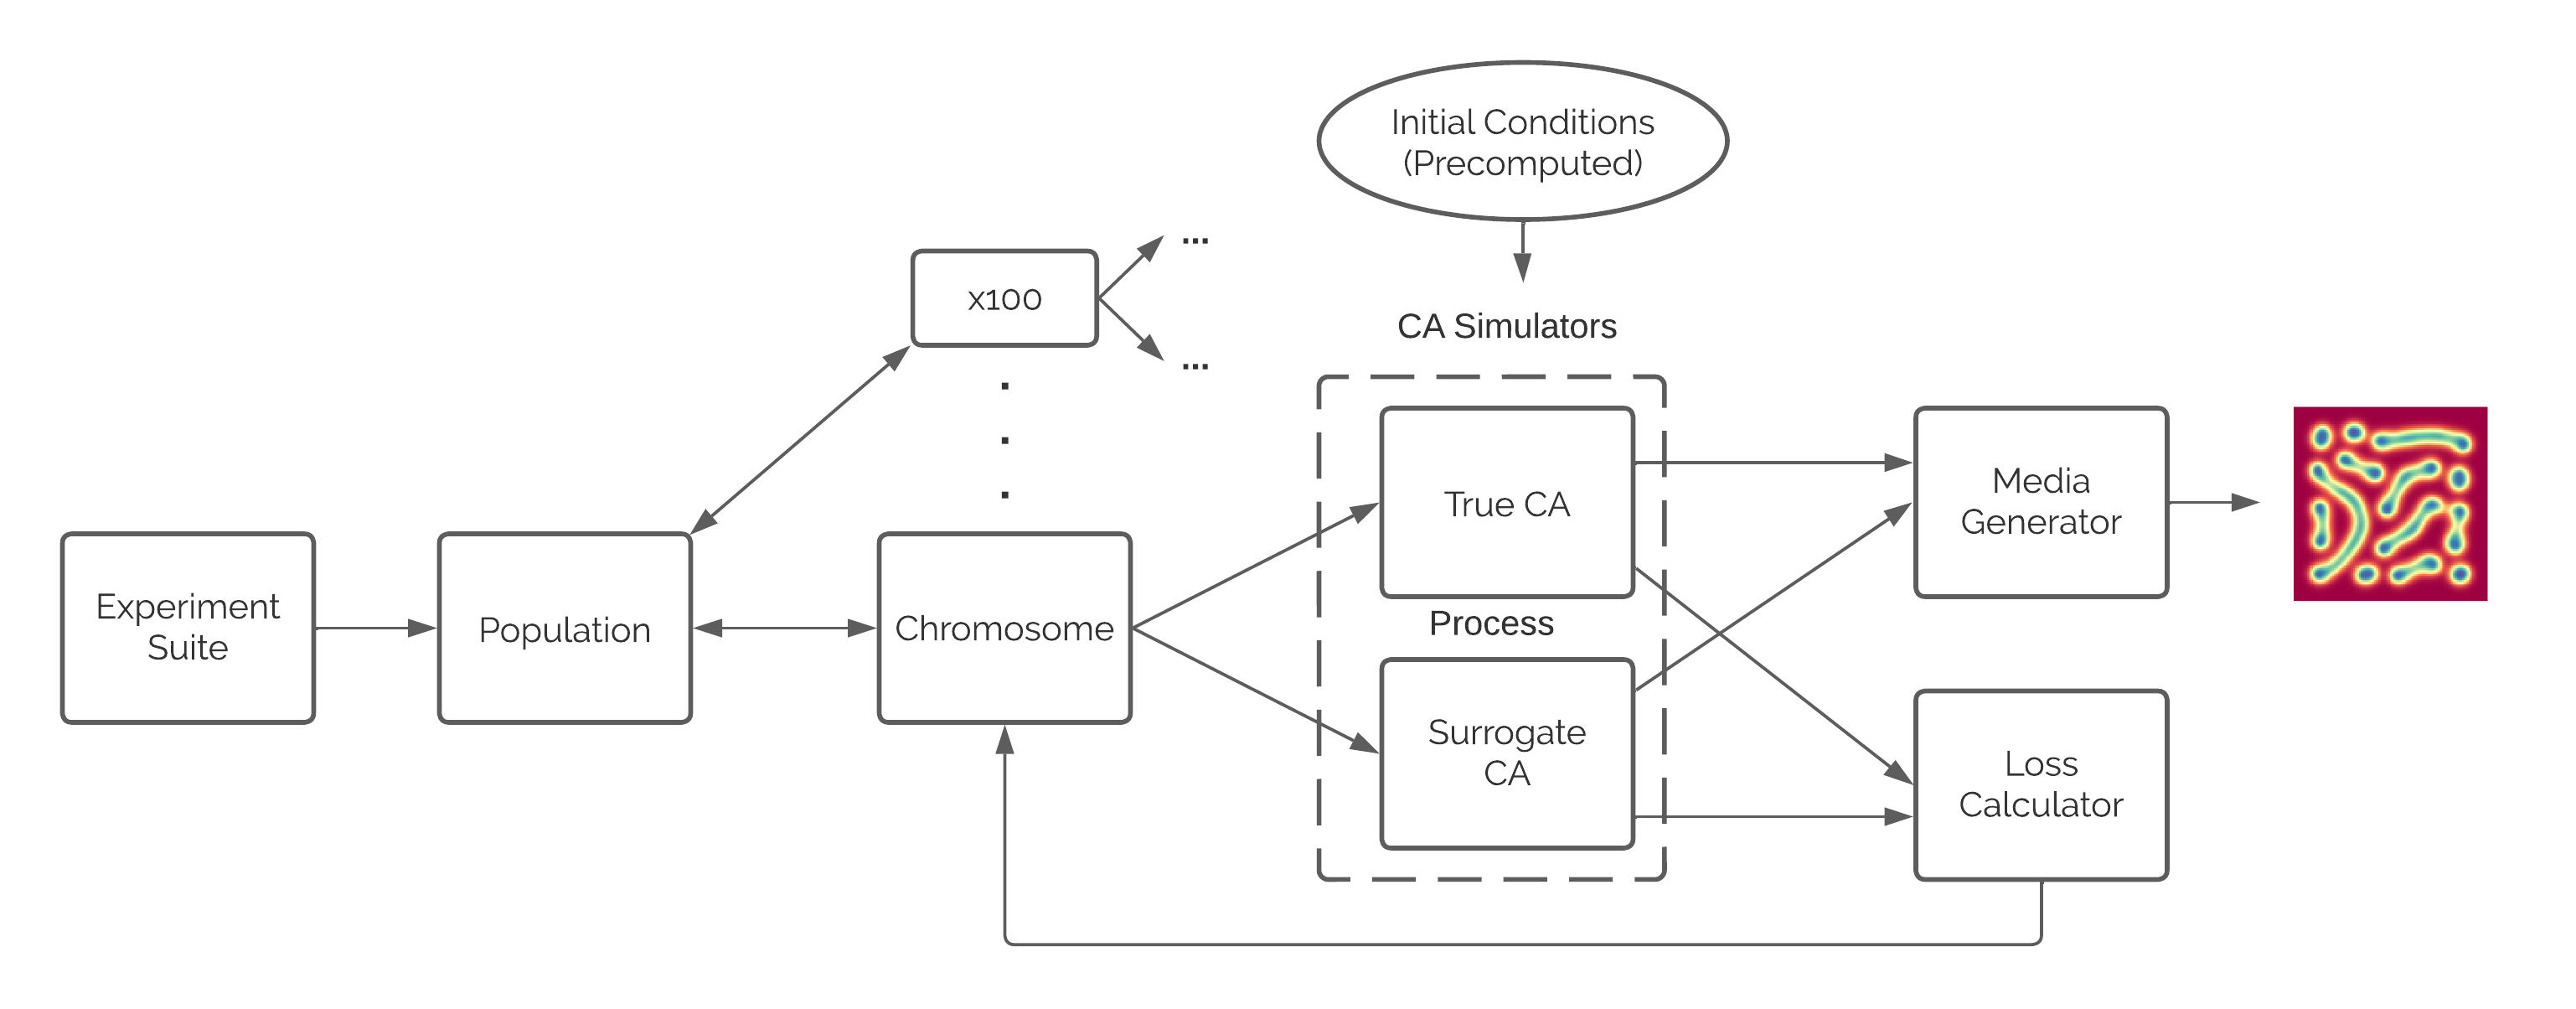
\includegraphics[width=\textwidth]{images/dataflow.png}
    \caption{Process for learning Life-Like and Gray-Scott CA}
\label{fig:dataflow}
\end{figure}

\section{Genetic Algorithm II} \label{sec:ga-2}

In this case, the optimization goal is to find the transition rule that generated the observations made. We maintain the same genetic operators as \nameref{sec:ga-1} using single point crossover and point mutation.\\

Selection comes in two flavours, \textit{plus} and \textit{comma}. Under  $(\mu + \lambda)$ plus-selection, we produce a population of $\lambda$ children from $\mu$ parents and the next generation is selected from the collective. Under $(\mu, \lambda)$ comma-selection, the next generation is selected exclusively from the $\lambda$ children. We can interpret this as an age restriction of 1 generation on the $\mu$ parent candidates. While this promotes exploration outside of local optima, it is easy for promising solutions to die out if they do not immediately pass on their advantageous characteristics to the next generation. This hinders convergence.\\

Fitness is calculated by running multiple simulations with the given transition function. For an $N \times N$ CA, it is infeasible to test on all $2^{N^2}$ initial conditions. Instead, a sample is picked. To ensure fairness, all CA are tested on the same set of initial conditions sampled uniformly on densities in $[0, 1]$.\todo{why} In order to learn full rule dynamics, we design a fitness function that quantifies the ability of a candidate to convert the state observed in the goal CA at time $t$ to the state observed at time $t+\delta$ over $\delta$ time steps. Suppose $K$ observations of the goal CA are made producing states $X_{\delta_1}, X_{\delta_2} ..., X_{\delta_K}$ where the number of time steps between $X_{\delta_k}$ and $X_{\delta_{k+1}}$ is $\delta_{k+1}$. We define the loss of a candidate between observations $k$ and $k+1$ as the mean number of differing states cell-wise between $X_{\delta_{k+1}}$ and $\phi^{\delta_{k+1}}(X_{\delta_k})$ which is the state of the candidate CA initialised at $X_{\delta_k}$ when observed $\delta_{k+1}$ time steps after initialisation. The loss between each observation is in $[0 ,1]$. The fitness is defined by taking the mean of the losses and subtracting from 1.

\begin{definition}[Life-Like Fitness Function 1]
We define the fitness $F$ as
\begin{align}
    F &= 1 - \bar{L}\\
    \textnormal{where\ } \bar{L} &= \frac{1}{N^2(K-1)}\sum_{k=1}^{K-1} \left| X_{\delta_{k+1}} \oplus \phi^{\delta_{k+1}}(X_{\delta_k}) \right|
\end{align}
where $\oplus$ is the XOR operator and we use $|X|$ to represent the number of living cells in state $X$.
\end{definition}

The number of observations and the values of the inter-observation times (or "step sizes") are hyperparameters. If $K$ is too high, we perform needless computations observing increasingly similar states as the CA stabilises. If $K$ is too low, we only observe early transient patterns instead of the long-lived patterns that characterise the objective rule. With regard to step sizes, we consider 3 possibilities.

\begin{enumerate}
    \item Constant: $\delta_1 = \delta_2 = ... = \delta_K = C$.
    \item Random Uniform: $\delta_k \sim \mathit{Uniform}(D_{min}, D_{max})$
    \item Random Increasing Uniform $\delta_k \sim \mathit{Uniform}(f_{min}(k), f_{max}(k))$\todo{Test this in evaluation}
\end{enumerate}

where $f_{min}$ and $f_{max}$ are monotonically increasing functions of $k$. While a constant stepsize is simpler to implement, a random uniform stepsize is less likely to conflate periodic patterns in the CA with convergence. For example, consider \textit{Fumarole}, a 5-period oscillator in the Game of Life shown in Figure~\ref{fig:fumarole}. If $C=5$, the loss at each observation would be calculated using only one of its states. A rule that supports a still-life of the same configuration would be considered as optimal as the true rule. On the contrary, a random uniform stepsize with $D_{min} < 5 < D_{max}$ is extremely unlikely to land on the same state each time. The chances of this are only
\begin{equation}
\left(\frac{1}{D_{max} - D_{min}}\right)^K
\end{equation}
Therefore, an algorithm with random uniform step size is much more likely to rank the true rule as fitter than the imposter. The random increasing uniform distribution goes a step further, increasing the expected value of $\delta_k$ as $k$ increases to allow time for late-stage patterns to appreciably change before making further observations.\\

\begin{figure}[!h]
\centering
            \subfloat{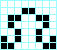
\includegraphics[width=.15\textwidth]{images/fumarole/0.png}}\hfill
            \subfloat{
\includegraphics[width=.15\textwidth]{images/fumarole/1.png}}\hfill
            \subfloat{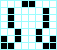
\includegraphics[width=.15\textwidth]{images/fumarole/2.png}}\hfill
            \subfloat{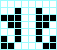
\includegraphics[width=.15\textwidth]{images/fumarole/3.png}}\hfill
            \subfloat{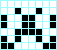
\includegraphics[width=.15\textwidth]{images/fumarole/4.png}}\hfill
            \caption{\textit{Fumarole}, a 5-period oscillator in the Game of Life. \cite{fumarole}}
\label{fig:fumarole}
\end{figure}

However, a fitness function that compares states cell-wise can be too fine-grained. It fails to capture macroscropic properties such as the density of live cells across different regions in the lattice. As a simple example, Figure~\ref{fig:singleres-fail} shows two predictions for a goal state. Prediction 1 clearly has a similar density and pattern to the goal but its live cells do not align with the live cells of the goal. Prediction 2 only has a single live cell making it quite different from the goal but due to the position of that cell, it achieves a much higher fitness than prediction 1. To mitigate this affect, a multi-resolution fitness function is proposed which uses convolutions to capture density across broad regions.\\

\begin{figure}[!h]
\centering
            \subfloat[Goal State]{
\includegraphics[width=.2\textwidth]{images/multires/1.png}}\hfill
            \subfloat[Prediction 1, fitness = 0]{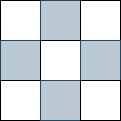
\includegraphics[width=.2\textwidth]{images/multires/2.png}}
            \hfill
            \subfloat[Prediction 2, fitness = 0.55]{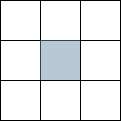
\includegraphics[width=.2\textwidth]{images/multires/3.png}}\hfill
            \caption{Example of fine-grain loss failing to capture macroscropic properties}
\label{fig:singleres-fail}
\end{figure}

\begin{definition}[Life-Like Fitness Function 2]
We define the multi-resolution fitness $F$ as
\begin{align}
    F &= 1 - \bar{L}\\
    \textnormal{where\ } \bar{L} &= \frac{1}{N^2M(K-1)} \sum_{k=1}^{K-1} \sum_{m=1}^{M} \left| \round{\omega_m \ast X_{\delta_{k+1}}} \oplus \round{\omega_m \ast \phi^{\delta_{k+1}}(X_{\delta_k})}\\
    \textnormal{where\ } \omega_m &= \frac{1}{m^2} \right|
    \begin{pmatrix}
        1 & \ldots & 1\\
        \vdots & \ddots & \vdots\\
        1 & \ldots & 1\\
    \end{pmatrix}
    \in \mathbb{R}^{m \times m}
\end{align}
where $\omega \ast f$ is a 2D convolution over image $f$ with filter kernel $\omega$ and $\round{.}$ is the integer rounding operator.
\end{definition}

The filter kernel used, $\omega_m$, is the all-ones matrix divided by the size of the kernel. This ensures that $\omega_m \ast X$ has entries between 0 and 1 and that, after rounding, the convolution is a binary matrix with each cell representing whether there are more live or dead cells in an $m \times m$ region of the lattice. After XORing and summation, the loss $\bar{L}$ is between 0 and 1 and so is the fitness.



\section{Software Engineering Design} \label{sec:sed}

Design decisions regarding algorithms and process have been discussed throughout Chapters \ref{procedural} and \ref{lifelike}. In this section, we summarise key software engineering design decisions when writing the evolutionary algorithm toolkit.\\

Figure~\ref{fig:uml-seq} depicts the sequence of events that is triggered in a typical experiment learning life-like CA. There are three major loops that run during an experiment. The outer loop performs generational learning where the population is updated on each iteration. The inner loop calculates loss where each of the two CA is stepped forward by a certain number of time steps on each iteration. SurrogateCA is a subclass of CA with a \texttt{step\_from} method that can set an explicit initial condition. This allows it to be reseeded with true data on each iteration of the inner loop. The final loop reruns top solutions to generate statistics and media.\\

\begin{figure}[!h]
\centering
    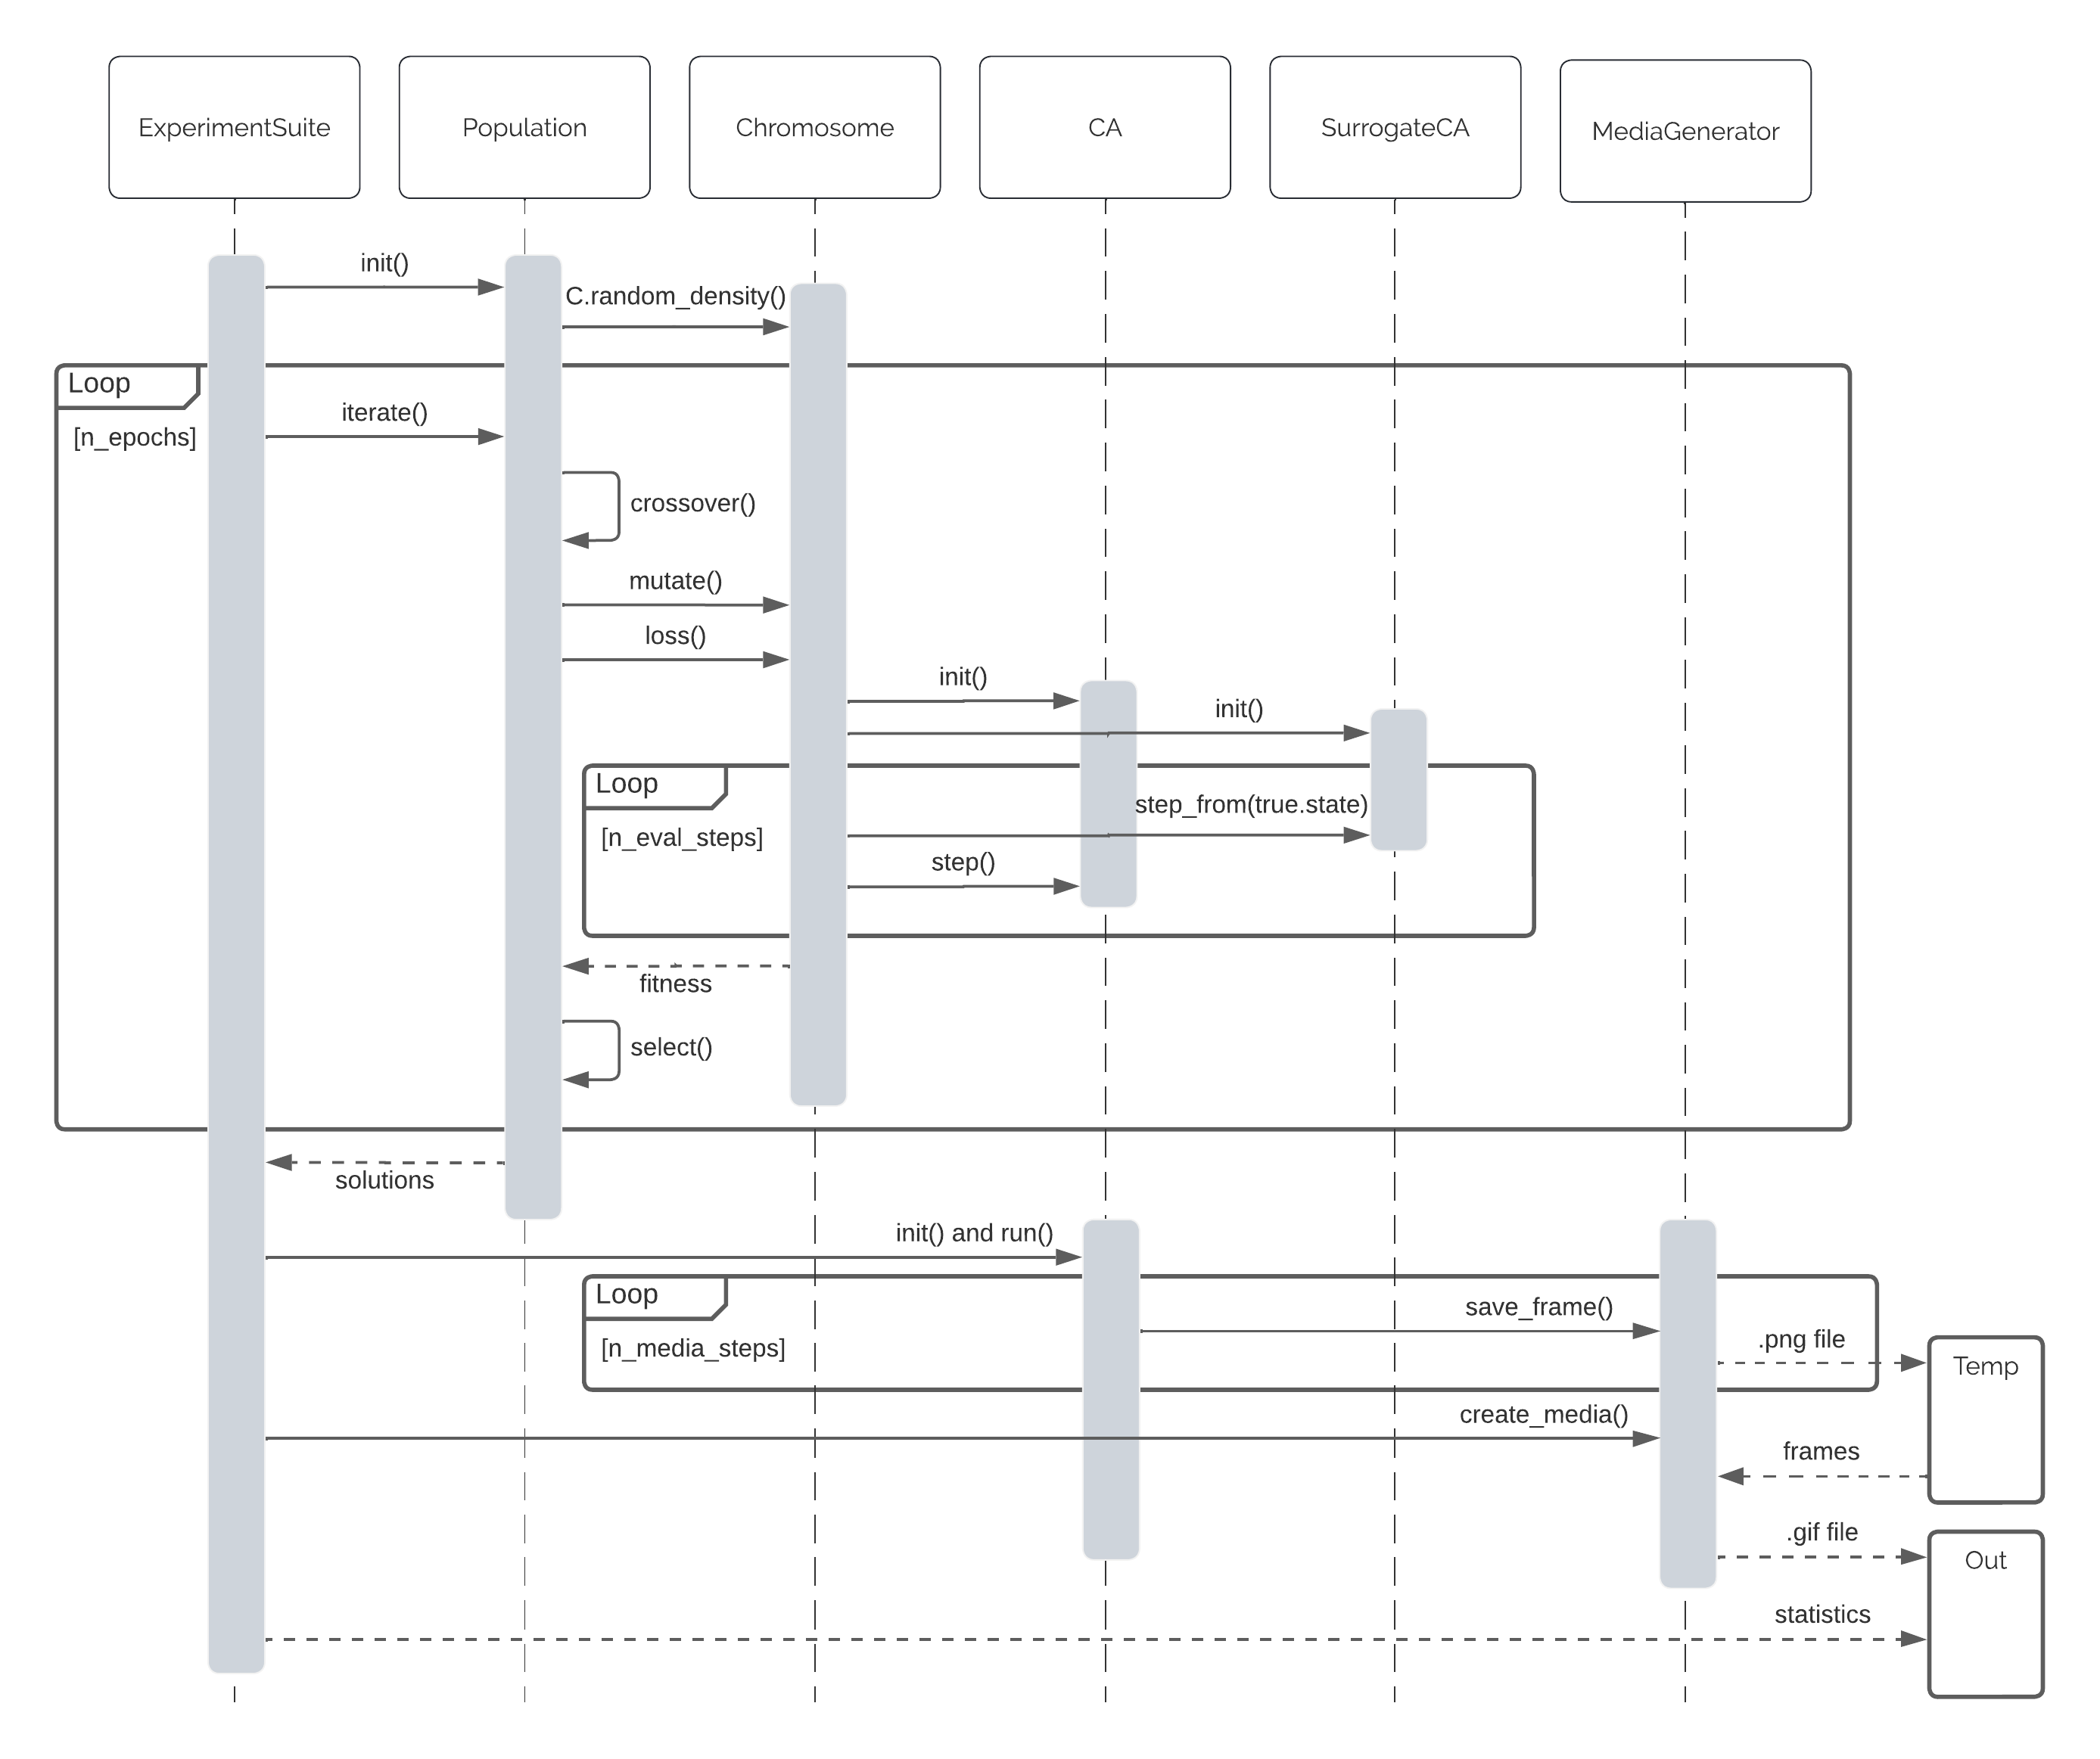
\includegraphics[width=\textwidth]{images/uml_seq.png}
    \caption{UML sequence diagram of life-like CA learning}
\label{fig:uml-seq}
\end{figure}

One notable decision is about changes to fields in the Chromosome class during operations like mutation and crossover. To avoid repeated calculations converting between birth/survival sets and binary rule strings, we write the Chromosome class to keep track of both formats simultaneously. However, this requirement means both sets must be updated every time the binary rule string is updated and vice versa. Although Python allows direct access to private class fields, it is verbose and error-prone to update all fields every time a single field needs to be changed. We automatically enforce synchronisation between these fields through using \texttt{@property} decorators. We define a setter method that updates the birth and survival sets every time the binary rule string is updated. By decorating this with \texttt{@property}, the setter is implicitly called every time a modification is made to the rule string field. We implement the same for the birth and survival sets too.\\

Another key decision was about initialisation. Two common initialisation methods for chromosomes are based on sampling uniformly across density, and sampling uniformly across value. By implementing both of these as factory methods, we create a extensible class where new initialisation methods can be easily implemented and tested. \texttt{Chromosome.random\_density()} and \texttt{Chromosome.random\_value()} are public factory methods that generate a binary rule string and call another internal factory method \texttt{Chromosome.from\_rstring()} which calculates the birth and survival sets then passes all three parameters to the main constructor which creates a new \texttt{Chromosome} object.\\

Metrics and media are generated to extract insights from the toolkit. The experiment suite class configures populations according to user-defined parameters and records metrics from the population at each epoch in Pandas dataframes. These metrics are saved to a .csv file at regular intervals so that data is partially logged if the program fails midway through an experiment. Media is generated automatically once an experiment has finished. The top 3 solutions are simulated again. During simulation, a media save is triggered at regular intervals whereby the state of the running CA is converted into a 2D regular raster graphic using Matplotlib and saved as a png file in a temporary folder. If there are multiple stages of simulation (e.g. growth, region find, and region merge), one temporary folder is created per stage. This simplifies the generation of animated gifs and promotes extensibility in case more stages are to be added in the future. After simulation, these images are stitched together into animations using the Python Imaging Library (PIL). The final state of each CA is also saved as a png image and in its original array form as a .npy file. The .npy file is saved in case a later analysis requires the CA to continue running from where it stopped. The temporary frame files are deleted to save memory. Analysis and visualisation of population-wide properties is done manually after the experiments.
